\documentclass{article}

\usepackage[top=3cm, bottom=3cm, left=3cm, right=3cm]{geometry}

\usepackage[utf8]{inputenc}
\usepackage[T1]{fontenc}
\usepackage[frenchb]{babel}

\usepackage[a4paper,colorlinks,linkcolor=darkgray,citecolor=red,urlcolor=blue]{hyperref}
\usepackage{graphicx}
\usepackage{caption}
\usepackage{subcaption}
\usepackage{amsthm}
\usepackage{listings}
\usepackage{tikz}
\usepackage{algorithm}
\usepackage{amsmath}
\usepackage[noend]{algpseudocode}
\usepackage{amsfonts}
\usepackage{amssymb}
\usepackage{authblk}

\usepackage{tikz} % Let us start the fun
\usetikzlibrary{positioning, chains, calc, arrows, decorations.pathreplacing, fit, patterns, snakes}

\makeatletter
 
\newskip\@bigflushglue \@bigflushglue = -100pt plus 1fil
 
\def\bigcenter{\trivlist \bigcentering\item\relax}
\def\bigcentering{\let\\\@centercr\rightskip\@bigflushglue%
\leftskip\@bigflushglue
\parindent\z@\parfillskip\z@skip}
\def\endbigcenter{\endtrivlist}
 
\makeatother

\renewcommand\Affilfont{\small}

\title{Projet Images}

\author[$\dag$]{Laureline Pinault et Raphaël Charrondière}
\affil[$\dag$]{ENS de Lyon, France}

\date{Lundi 4 mai 2015}

\begin{document}

  \maketitle

  \begin{abstract}
   
  \end{abstract}
  
  \newpage

  \tableofcontents

  \newpage
  
  \section{Introduction}
  
    \subsection{Remarques préliminaires}
    
    \subsection{Objectifs du projet}
  
    \subsection{Organisation du projet} %TODO : Raphaël
  
  \section{Traitement des images}
  
    \subsection{Traitement anti-inversion}
    
      \begin{figure}[!h]
	\centering
	\begin{subfigure}{.49\textwidth}
	  \begin{subfigure}{.49\textwidth}
	    \centering
	    \includegraphics[scale=0.25]{Illustrations/rat-8.png}
	    \label{1strat}
	  \end{subfigure}
	  \begin{subfigure}{.49\textwidth}
	    \centering
	    \includegraphics[scale=0.25]{Illustrations/rat-8-inverse.png}
	    \label{1strat-inverse}
	  \end{subfigure}
	  \subcaption{Ce rat n'a pas été inversé}
	\end{subfigure}
	\begin{subfigure}{.49\textwidth}
	  \begin{subfigure}{.49\textwidth}
	    \centering
	    \includegraphics[scale=0.25]{Illustrations/rat-9.png}
	  \label{2ndrat}
	  \end{subfigure}
	  \begin{subfigure}{.49\textwidth}
	    \centering
	    \includegraphics[scale=0.25]{Illustrations/rat-9-inverse.png}
	  \label{2ndrat-inverse}
	  \end{subfigure}
	  \subcaption{Ce rat a été inversé}
	\end{subfigure}
	\caption{Inversion de l'objet rat}
	\label{anti-inversion}
      \end{figure}

    \subsection{Normalisation des images}     %TODO : Raphaël
      
    \subsection{Traitement anti-bruit}
    
    \subsection{Remplissage}
    
      \begin{figure}[!h]
	\centering
	\begin{subfigure}{.25\textwidth}
	  \centering
	  \includegraphics[scale=0.30]{Illustrations/pocket-20.png}
	  \label{pocket-non-rempli}
	\end{subfigure}
	\begin{subfigure}{.25\textwidth}
	  \centering
	  \includegraphics[scale=0.30]{Illustrations/pocket-20-rempli.png}
	\label{pocket-rempli}
	\end{subfigure}
	\caption{Remplissage de l'objet pocket}
	\label{remplissage}
      \end{figure}
      
      \begin{figure}[!h]
	\centering
	\begin{subfigure}{.47\textwidth}
	  \begin{subfigure}{.52\textwidth}
	    \centering
	    \includegraphics[scale=0.295]{Illustrations/butterfly-10-rempli.png}
	    \label{butterfly-rempli}
	  \end{subfigure}
	  \begin{subfigure}{.45\textwidth}
	    \centering
	    \includegraphics[scale=0.16]{Illustrations/device9-6-rempli.png}
	    \label{spirale-rempli}
	  \end{subfigure}
	  \subcaption{Certains détails ne sont pas remplis}
	\end{subfigure}
	\begin{subfigure}{.44\textwidth}
	  \begin{subfigure}{.46\textwidth}
	    \centering
	    \includegraphics[scale=0.25]{Illustrations/cup-7-rempli.png}
	  \label{1stcup-rempli}
	  \end{subfigure}
	  \begin{subfigure}{.46\textwidth}
	    \centering
	    \includegraphics[scale=0.275]{Illustrations/cup-12-rempli.png}
	  \label{2ndcup-rempli}
	  \end{subfigure}
	  \subcaption{Les tasses ne sont pas remplies pareil}
	\end{subfigure}
	\caption{Problèmes soulevés par le remplissage des objets}
	\label{problèmes-remplissage}
      \end{figure}      
   
  \section{Estimateurs}
  
    \subsection{Quelques estimateurs simples et complémentaires}

      \subsubsection{Solidité}
      
	\paragraph{Principe}
	
	  \begin{figure}[!h]
	    \centering
	    \begin{subfigure}{.25\textwidth}
	      \centering
	      \includegraphics[scale=0.30]{Illustrations/horse-20.png}
	      \label{horse}
	    \end{subfigure}
	    \begin{subfigure}{.25\textwidth}
	      \centering
	      \includegraphics[scale=0.30]{Illustrations/horse-20-rempli-convexhull.png}
	    \label{horse-rempli-convexhull}
	    \end{subfigure}
	    \caption{Solidité de l'objet horse}
	    \label{solidité}
	  \end{figure}
	
	\paragraph{Programmation}
	
	\paragraph{Résistance aux inversions de couleur}
	
	\paragraph{Résistance au bruit}
	
	\paragraph{Résistance aux rotations et symmétries}
      
	\paragraph{Résistance aux homothéties} blabla \\
	
	  \begin{table}
	  \centering
	  \begin{tabular}{|c|c|c|c|c|c|c|c|}
	    \hline
	    \multicolumn{2}{|c|}{Cheval} & \multicolumn{2}{|c|}{Pomme} & \multicolumn{2}{|c|}{Device} & \multicolumn{2}{|c|}{Lézard} \\
	    \multicolumn{2}{|c|}{\includegraphics[scale=0.15]{Illustrations/horse-20.png}} 
	    & \multicolumn{2}{|c|}{\includegraphics[scale=0.15]{Illustrations/apple-3.png}} 
	    & \multicolumn{2}{|c|}{\includegraphics[scale=0.075]{Illustrations/device7-1.png}} 
	    & \multicolumn{2}{|c|}{\includegraphics[scale=0.09]{Illustrations/lizzard-13.png}} \\
	    \hline
	    \textbf{Echelle} & \textbf{Solidité} & \textbf{Echelle} & \textbf{Solidité} & \textbf{Echelle} & \textbf{Solidité} & \textbf{Echelle} & \textbf{Solidité} \\
	    \hline
	    0.5 & 0.584583 & 0.5 & 0.933504 & 0.5 & 0.77016 & 0.5 & 0.767554 \\
	    \hline
	    1 & 0.577491 & 1 & 0.931911 & 1 & 0.768281 & 1 & 0.762166 \\
	    \hline
	    2 & 0.57244 & 2 & 0.930546 & 2 & 0.767288 & 2 & 0.75678 \\
	    \hline
	    5 & 0.569273 & 5 & 0.929267 & 5 & 0.703692 & 5 & 0.7533 \\
	    \hline
	  \end{tabular}
	  \caption{Variations de la solidité de plusieurs objets selon l'agrandissement}
	  \label{solidité-scaling-table}
	  \end{table}
	  
	\paragraph{Résistance aux élongations}
	
	\paragraph{Résistance aux occlusions}
	  
	\paragraph{Résultats}
	
	  \begin{figure}[!h]
	    \begin{bigcenter}
	      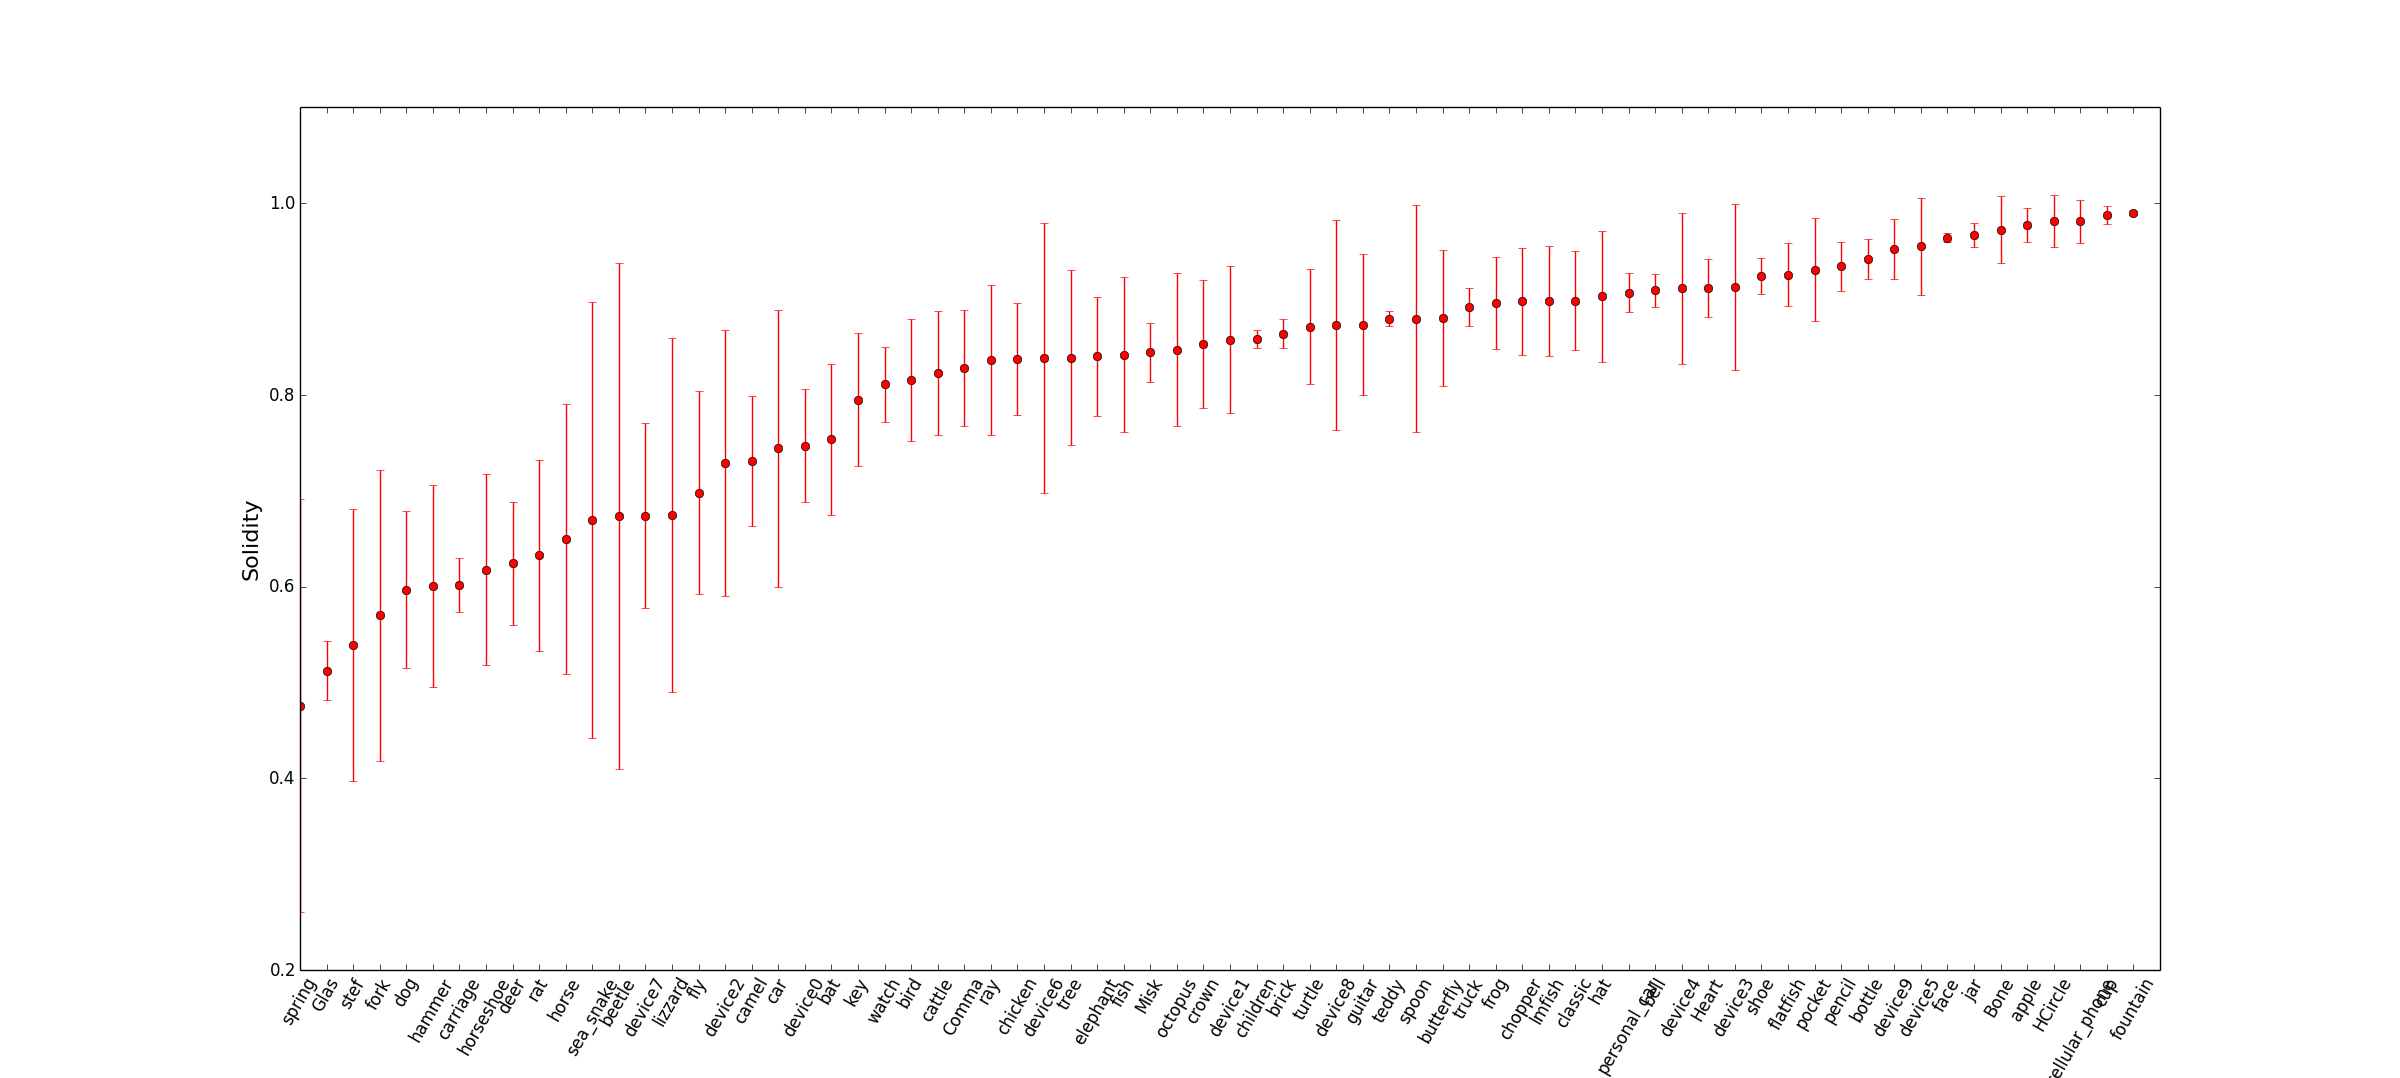
\includegraphics[scale=0.38]{Graphes/solidite.png}
	    \end{bigcenter}
	    \caption{Moyenne et écart type de la solidité pour chaque classe}
	    \label{solidité}
	  \end{figure}

      \subsubsection{Excentricté}
      
	\paragraph{Principe}
      
	\paragraph{Programmation}
	
	\paragraph{Résistance aux inversions de couleur}
	
	\paragraph{Résistance au bruit}
	
	\paragraph{Résistance aux rotations et symmétries}
      
	\paragraph{Résistance aux homothéties} blabla
	
	
	  \begin{table}
	  \centering      
	  \begin{tabular}{|c|c|c|c|c|c|}
	    \hline
	    \multicolumn{2}{|c|}{Chauve-souris} & \multicolumn{2}{|c|}{Marteau} & \multicolumn{2}{|c|}{Device}  \\
	    \multicolumn{2}{|c|}{
\includegraphics[scale=0.11]{Illustrations/bat-2.png}} 
	    & \multicolumn{2}{|c|}{
\includegraphics[scale=0.15]{Illustrations/hammer-20.png}} 
	    & \multicolumn{2}{|c|}{
\includegraphics[scale=0.07]{Illustrations/device9-9.png}}  \\
	    \hline
	    \textbf{Echelle} & \textbf{Excentricité} & \textbf{Echelle} & \textbf{Excentricité} & \textbf{Echelle} & \textbf{Excentricité} \\
	    \hline
	    0.5 & 2.32927 & 0.5 & 2.92308 & 0.5 & 1.0101 \\
	    \hline
	    1 & 2.33841 & 1 & 2.89873 & 1 & 1.01515 \\
	    \hline
	    2 & 2.33994 & 2 & 2.91772 & 2 & 1.01641 \\
	    \hline
	    5 & 2.34065 & 5 & 2.92152 & 5 & 1.01767 \\
	    \hline
	  \end{tabular}
	  \caption{Variations de l'excentricité de plusieurs objets selon l'agrandissement}
	  \label{excentricité-scaling-table}
	  \end{table}  
	  
	\paragraph{Résistance aux élongations}
	
	\paragraph{Résistance aux occlusions}
	  
	\paragraph{Résultats}
	  

      
      \subsubsection{Energie de flexion moyenne}
      
	\paragraph{Principe}
	
	\paragraph{Programmation}
	
	  Méthode du cercle circonscrit par les deux demis tangentes.
	  
	  \begin{figure}[!h]
	    \centering
	    \begin{tikzpicture}
	    \begin{scope}[scale = .4]
	      \draw (0,0) circle (5);
	      \node[] at (30:5) (Q) {\textbullet};
	      \node[right=.01cm of Q] {$Q$};
	      \node[] at (80:5) (P) {\textbullet};
	      \node[above=.01cm of P] {$P$};
	      \node[] at (165:5) (O) {\textbullet};
	      \node[left=.01cm of O] {$O$};
	      \draw[] (30:5) -- (80:5) -- (165:5) -- (30:5);
	      \node[] (C) {$\times$};
	      \node[below right=.01cm and .01cm of C] {$C$};
	      \draw[dashed] (0,0) -- node[right]{$r$} (80:5);
	    \end{scope}
	    \end{tikzpicture}
	    \caption{Cercle circonscrit au triangle OPQ}
	    \label{cercle-circonscrit}
	  \end{figure}
	  
	  Par la loi des sinus, $r = \frac{|QO|}{2 \sin\left(\widehat{OPQ}\right)}$. On en déduit que :
	  
	  \[ r = \frac{|QO|}{2 \sin\left(\widehat{OPQ}\right)} = \frac{|QO|}{\frac{2 \det\left(\overrightarrow{PO}, \overrightarrow{PQ} \right)}{|OP| |PQ|}} = \frac{|OP| |PQ| |QO|}{4 \mathcal{A}_{PQO}}  \]
	
	\paragraph{Résultats}
    
    \subsection{Transformée de Fourier}  %A mettre ? RAphaël
    
    \subsection{Méthode des moments} %A renommer ? Raphaël
    
    \subsection{Etude du squelette} %TODO : Raphaël
    
    \subsection{Pistes non explorées}
  
  \section{Résultats} 
  
    \subsection{Méthodologie d'estimation}  %En gros : c'est quoi nos résultats ?, je sais pas trop comment le nommer
    
    \subsection{Résultats} %Beaucoup de section / subsection = résultats
  
  \section{Conclusion}
  
\end{document}

